\documentclass{article}

% Language setting
% Replace `english' with e.g. `spanish' to change the document language
\usepackage[french]{babel}
\usepackage[fleqn]{amsmath} % Aligner les équations à gauche


% Set page size and margins
% Replace `letterpaper' with`a4paper' for UK/EU standard size
\usepackage[letterpaper,top=2cm,bottom=2cm,left=3cm,right=3cm,marginparwidth=1.75cm]{geometry}

% Useful packages

\usepackage{amsmath}
\usepackage{graphicx}
\usepackage{subcaption}
\usepackage[colorlinks=true, allcolors=blue]{hyperref}

\title{TD 11 - Ondes électromagnétiques suite}
\author{IPESUP - PC }
\date{04/12/2024}

\begin{document}
\maketitle

\section{Rappels de cours}

Conductivité complexe : $\underline{\gamma} = \frac{\gamma_0}{1 + i \omega \tau}$\\

Equation de propagation : $\Delta {\vec{E}} = \mu_0 \frac{\partial \vec{j}}{\partial t } + \frac{1}{c^2} \frac{\partial^2 \vec{E}}{\partial t^2}$ \\

Relation de dispersion dans un conducteur : $\underline{k}^2 = \frac{\omega^2}{c^2} - i \frac{\mu_0 \gamma_0 \omega}{1 + i \omega \tau}$:\\[0.2cm]
\textbf{Capacités exigibles}: \\
\begin{enumerate}
  \item Retrouver la conductivité complexe à partir du PFD à un électron. 
  \item Retrouver l'équation de propagation dans un conducteur.
  \item Retrouver la relation de dispersion dans un conducteur. 
  \item Effet de peau. 
\end{enumerate}




\section{Pression de radiation}

\begin{enumerate}
    \item Soit une onde plane, monochromatique, de fréquence $\nu$ se propageant le long des x croissants, dont le champ électrique est $\vec{E}(x,t)=E_0cos(\omega t-kx)\vec{u_y}$. Soit  $\mathcal{E}$ l'éclairement (défini par la puissance moyenne qui traverse une surface d'aire unité perpendiculaire à la direction de propagation). Exprimer $\mathcal{E}$ en fonction de $\epsilon_0, c $ et $E_0$. 
    \item On considère cette onde comme un faisceau de photons se propageant le long des x croissants. 
    \begin{enumerate}
        \item Exprimer $N_0$ le nombre de photons traversant par unité de temps l'unité de surface perpendiculaire à $Ox$ en fonction de $\mathcal{E}$ et de $\nu$. 
        \item L'onde arrive sur une surface plane perpendiculaire à $Ox$, d'aire S, et parfaitement réfléchissante. On étudie le rebondissement des photons sur cette surface. 
        \\
        Quelle est la quantité de mouvement reçue par la paroi au cours d'un choc photon-paroi ? \\
        Quelle est la force subie par la paroi en fonction de $\mathcal{E}$, $S$ et $c$ ? 
        Exprimer la pression $p$ subie par la paroi en fonction de $\mathcal{E}$ et $c$ puis en fonction de $\epsilon_0$ et $E_0$. 
        \item Reprendre la question ci-dessus lorsque la paroi est parfaitement aborbante. 
        \item Calculer $\mathcal{E}$, $E_0$ et $p$ sur une paroi totalement absorbante pour un laser ayant un diamètre $d$=5,00 mm et une puissance moyenne $\mathcal{P}$=100 W (laser utilisé industriellement pour la découpe de feuilles). 
    \end{enumerate}
    \item 
    \begin{enumerate} 
    \item L'onde est maintenant absorbée par une sphère de rayon $a$, bien inférieur au rayon du faisceau. Quelle est, en fonction de $\mathcal{E}$, $E_0$ et $p$, la force $\vec{F}$ subie par la sphère ? 
    \item Le soleil donne au voisinage de la Terre l'éclairement $\mathcal{E}$ = 1,4 $\times 10^3 W.m^{-2}$. L'émission est isotrope. Sur une surface de dimensions petites devant D, l'onde arrivant du Soleil est quasi plane. \\
    Quelle est la puissance $\mathcal{P_0}$ émise par le Soleil ? \\
    Un objet sphérique de rayon $a$, de masse volumique $\mu$ est situé à une distance $r$ du Soleil et absorbe totalement le rayonnement solaire. Evaluer le rapport entre la force due à l'absorbtion du rayonnement solaire et a force gravitationelle exercée par le Soleil sur cet objet dans les deux cas suivants:\\
    - Cas d'une météorite : $\mu = 3,0\times10^3 kg.m^{-3}$ et $a=1,0m$\\
    - Cas d'une poussière interstellaire: $\mu=1,0\times10^3kg.m^{-3}$
    \\ Commenter.
    \item Quelle est la surface minimale de la voile solaire d'un vaisseau spatial pour que celui-ci quitte l'attraction solaire ?  \\[2cm]
    \end{enumerate}
\end{enumerate}

\section{Onde longitudinale dans un plasma}

On étudie la propagation d'une onde électromagnétique dans un plasma peu dense. \\
On pose $\vec{E} = \vec{E}_0 exp(i(\omega t - \vec{k} \cdot \vec{r}))$ et $\vec{B} = \vec{B}_0 exp(i(\omega t - \vec{k} \cdot \vec{r} ))$
On suppose $\rho$ non nul. 

\begin{enumerate}
  \item Etablir l'équation du mouvement d'un électron de masse $m_e$ et de charge $-e$, associé à la densité $n_e$. Définir la conductivité complexe $\underline{\gamma}$ du plasma. 
  \item A l'aide des équations de Maxwell et de l'équation de conservation de la charge, établir une nouvelle expression de $\gamma$ en fonction de $\omega$ et $\epsilon_0$. 
  \item Montrer que $\vec{B}=0$ et en déduire que $\vec{E}$ est longitudinal. \\[2cm]
\end{enumerate}

\begin{figure}[h]
  \centering
  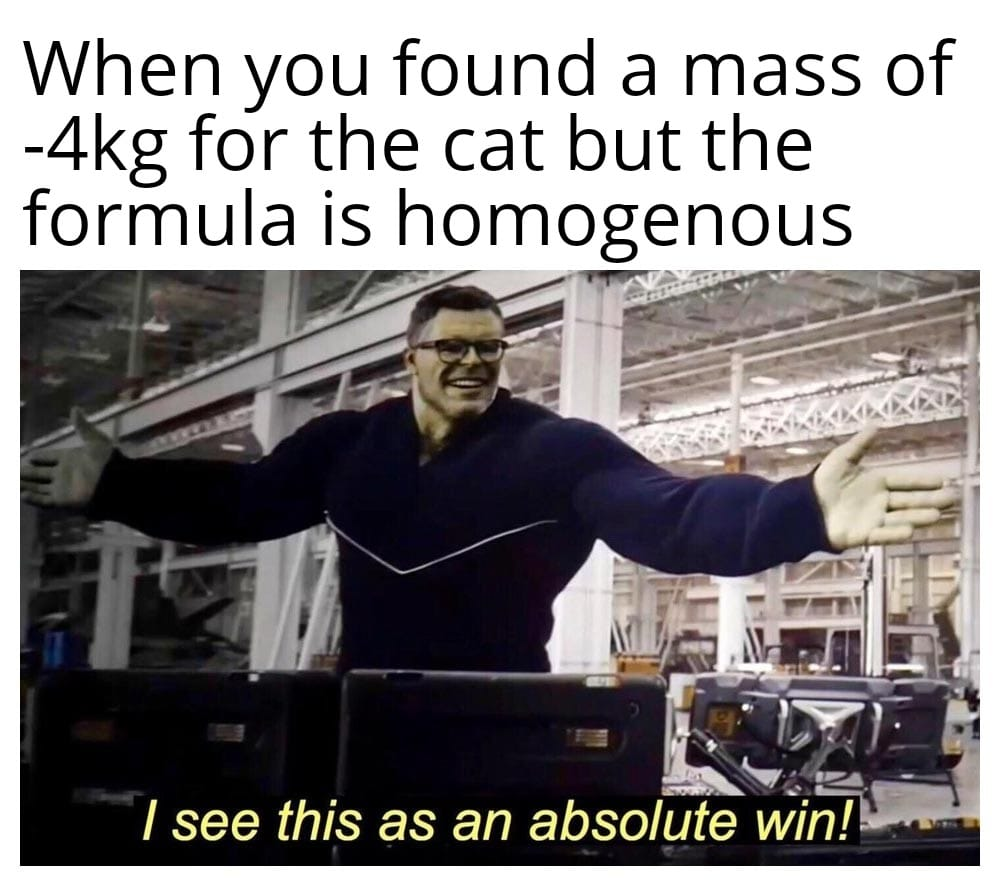
\includegraphics[width=0.4\textwidth]{meme.jpg}
  % \label{fig:schéma_guide_'ondes}
\end{figure}


% \section{Interro}

% On considère une OPPH se propageant dans le vide, dont la forme complexe est donéne par $\vec{\underline{E}}(M, t) = \vec{\underline{E}}_0 exp(i(\omega t - k x))$. 
% \begin{enumerate}
%   \item Dans quelle direction se propage l'onde ? 
%   \item Donner l'équation d'Alembert. 
%   \item Donner la relation de structure pour une OPPH. 
%   \item Calculer $\vec{\underline{B}}$. 
%   \item Retrouver la relation de dispersion de l'OPPH et en déduire la vitesse de phase et la vitesse de groupe. \\[1cm]
% \end{enumerate}


\end{document}













\end{document}
